\section{A9G2}
%A9G2
\begin{figure}[H]
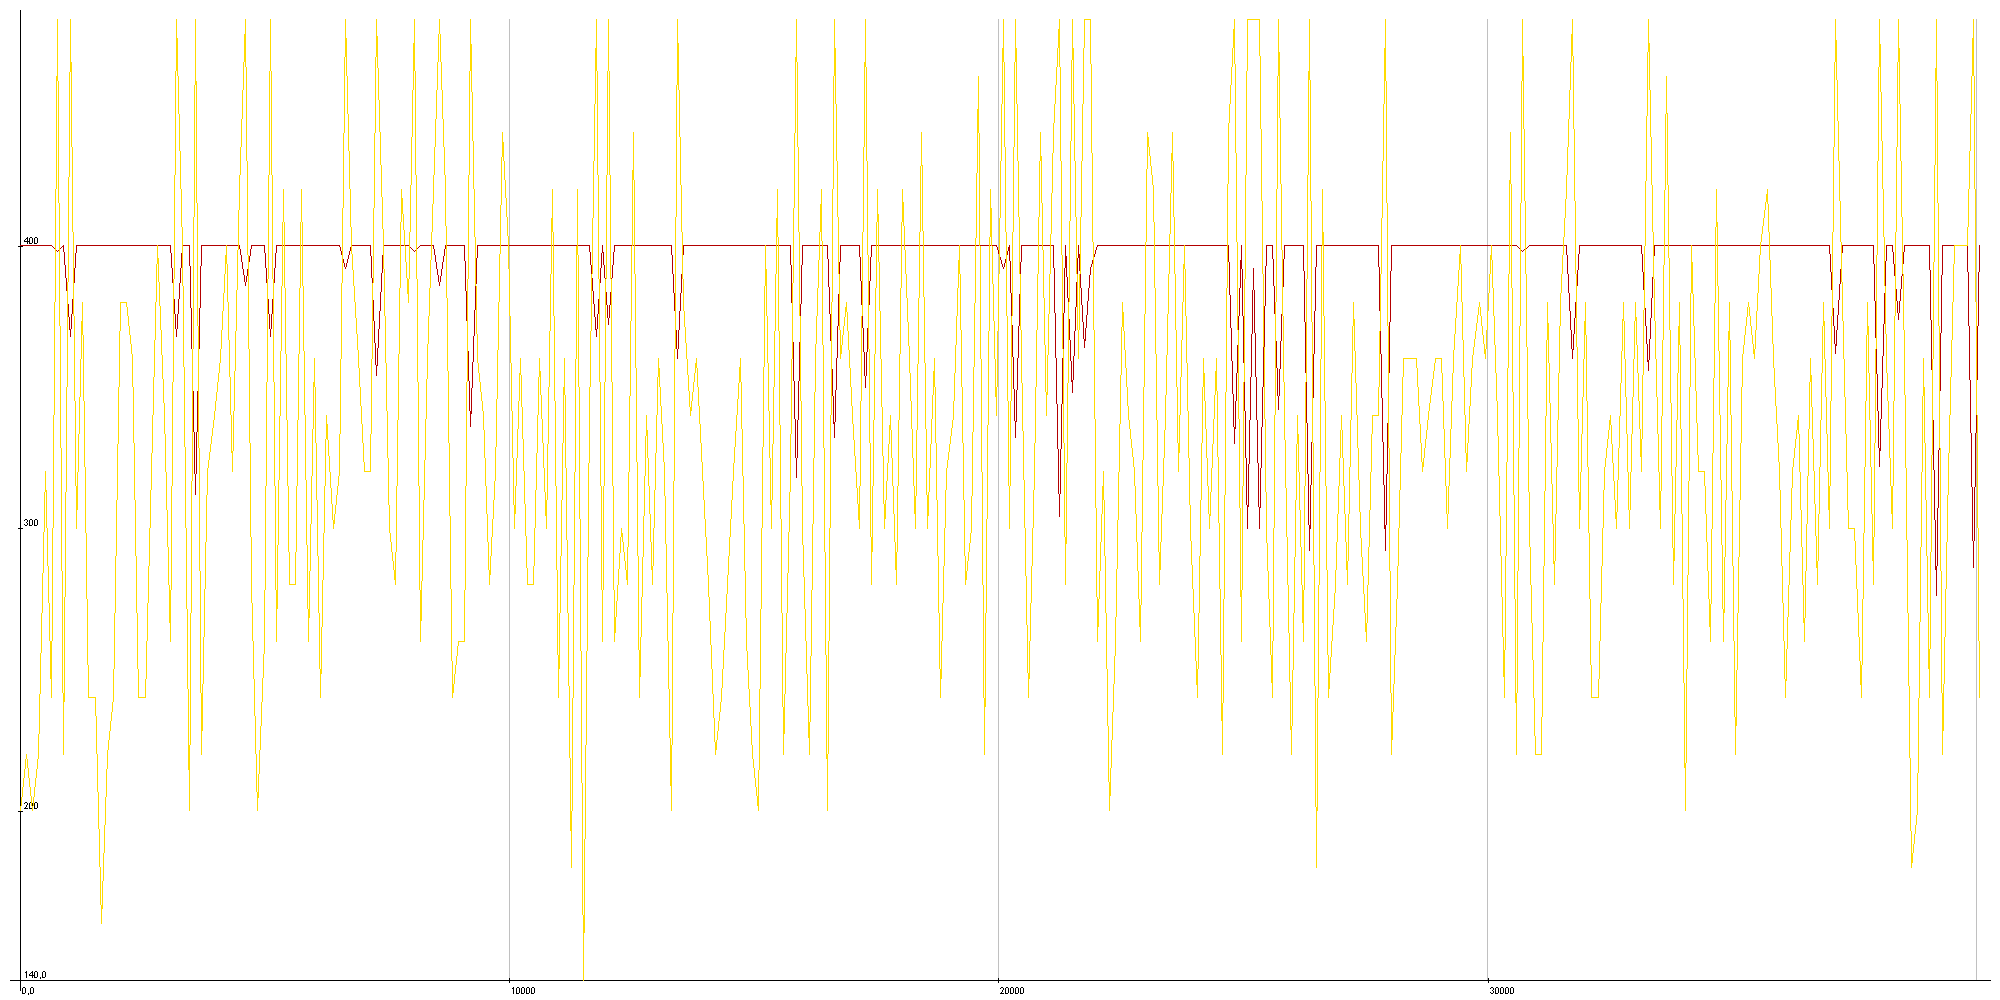
\includegraphics[angle=-90, scale=0.30]{Figures/learningrate/A9G2/damage.png}
\caption{Alpha 9 Gamma 2 damage - Blue: Damage given - Red: Damage taken}
\label{fig:app_a9g2_damage}
\end{figure}


\begin{figure}[H]
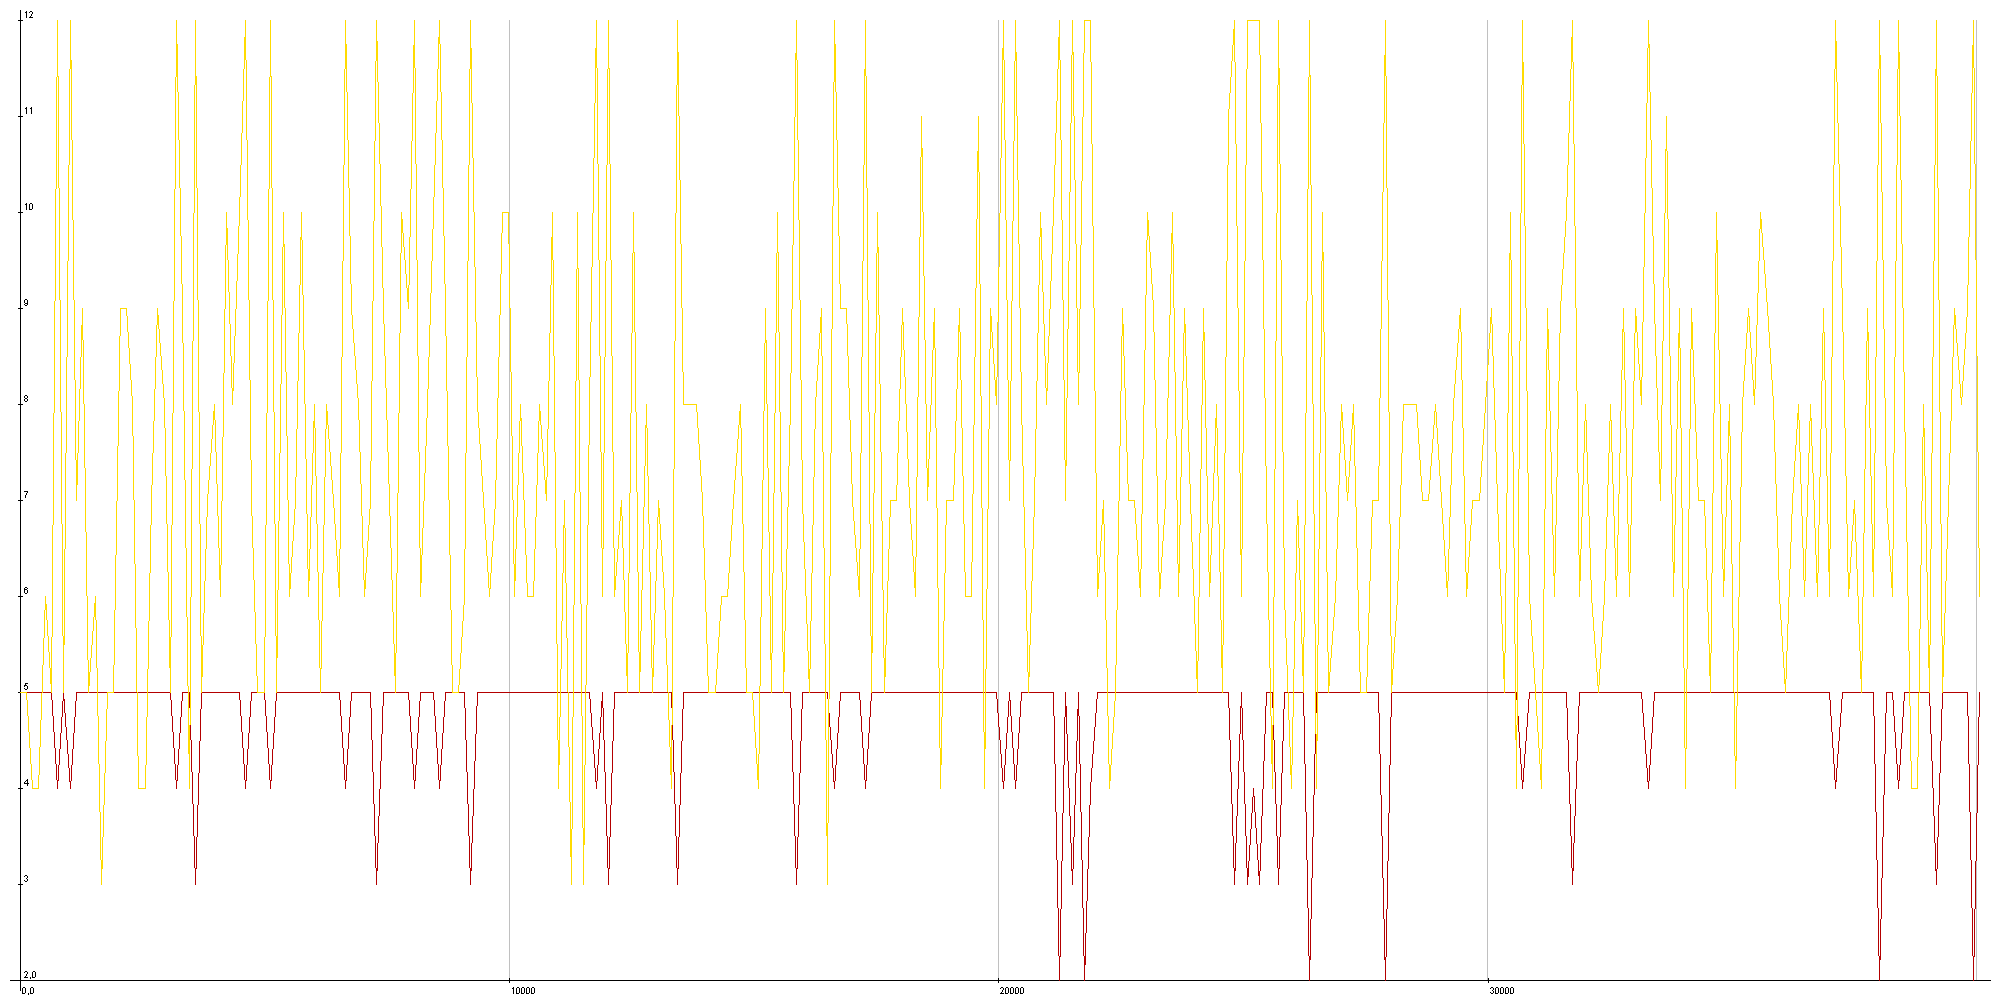
\includegraphics[angle=-90, scale=0.25]{Figures/learningrate/A9G2/units_lost_and_killed.png}
\caption{Alpha 9 Gamma 2 units lost and killed - Blue: Enemies killed - Red: Units lost}
\label{fig:app_a9g2_lak}
\end{figure}
	
\section{A6G4}
%A6G4	
\begin{figure}[H]
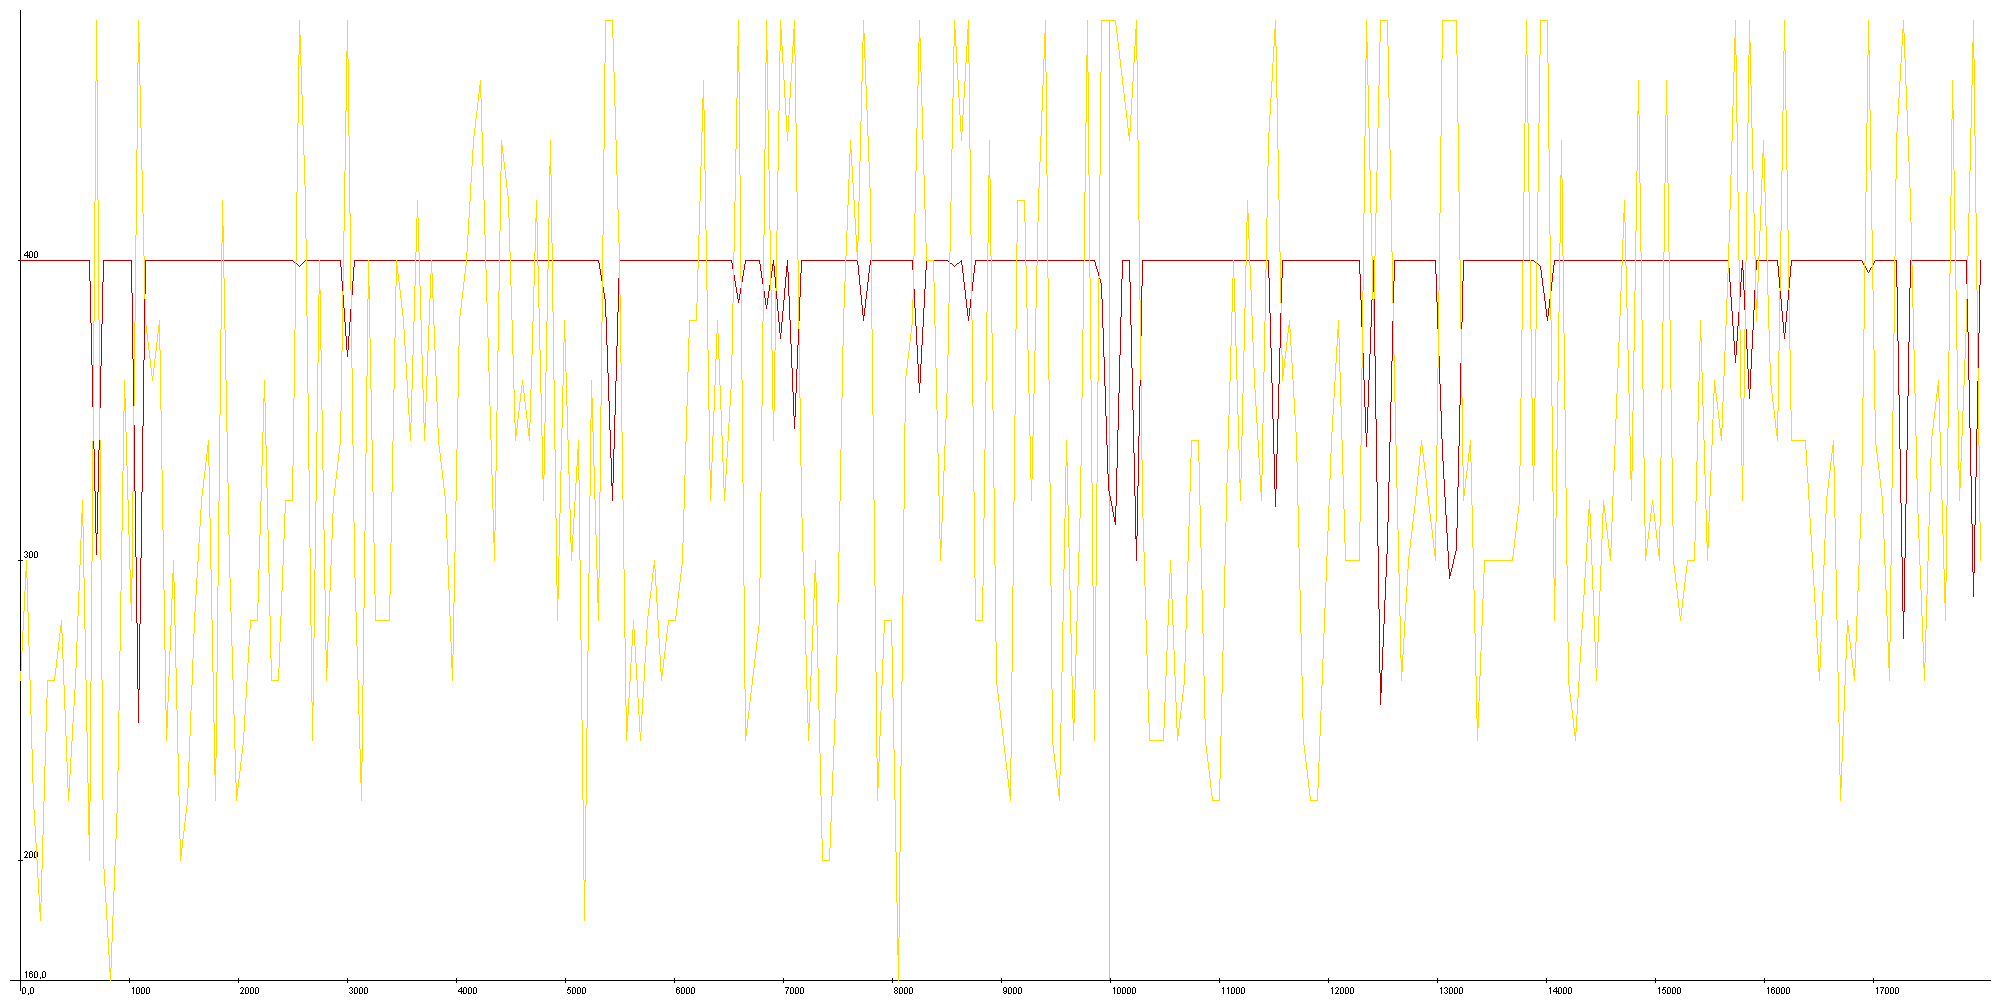
\includegraphics[angle=-90, scale=0.25]{Figures/learningrate/A6G4/damage.png}
\caption{Alpha 6 Gamma 4 damage - Blue: Damage given - Red: Damage taken}
\label{fig:app_a6g4_damage}
\end{figure}	
			

\begin{figure}[H]
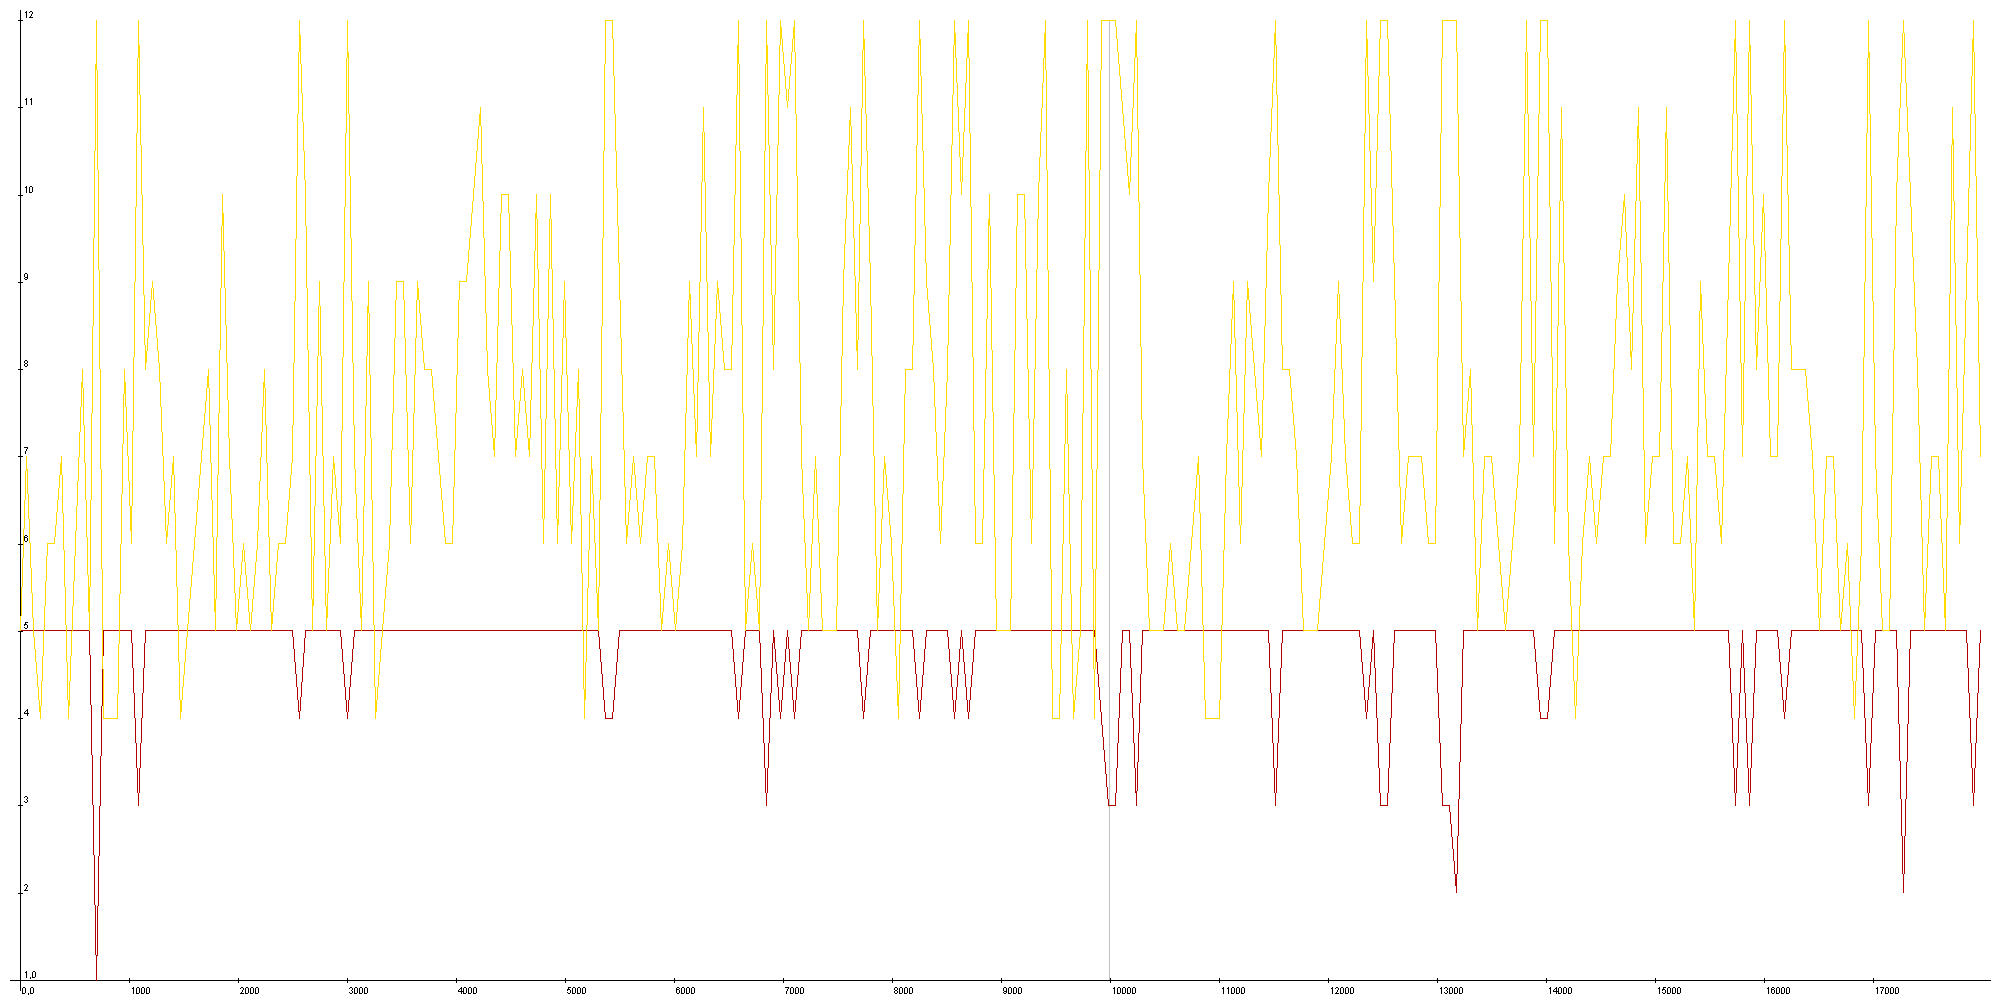
\includegraphics[angle=-90, scale=0.25]{Figures/learningrate/A6G4/units_lost_and_killed.png}
\caption{Alpha 6 Gamma 4 units lost and killed - Blue: Enemies killed - Red: Units lost}
\label{fig:app_a6g4_lak}
\end{figure}	


\section{A4G6}
%A4G6
\begin{figure}[H]
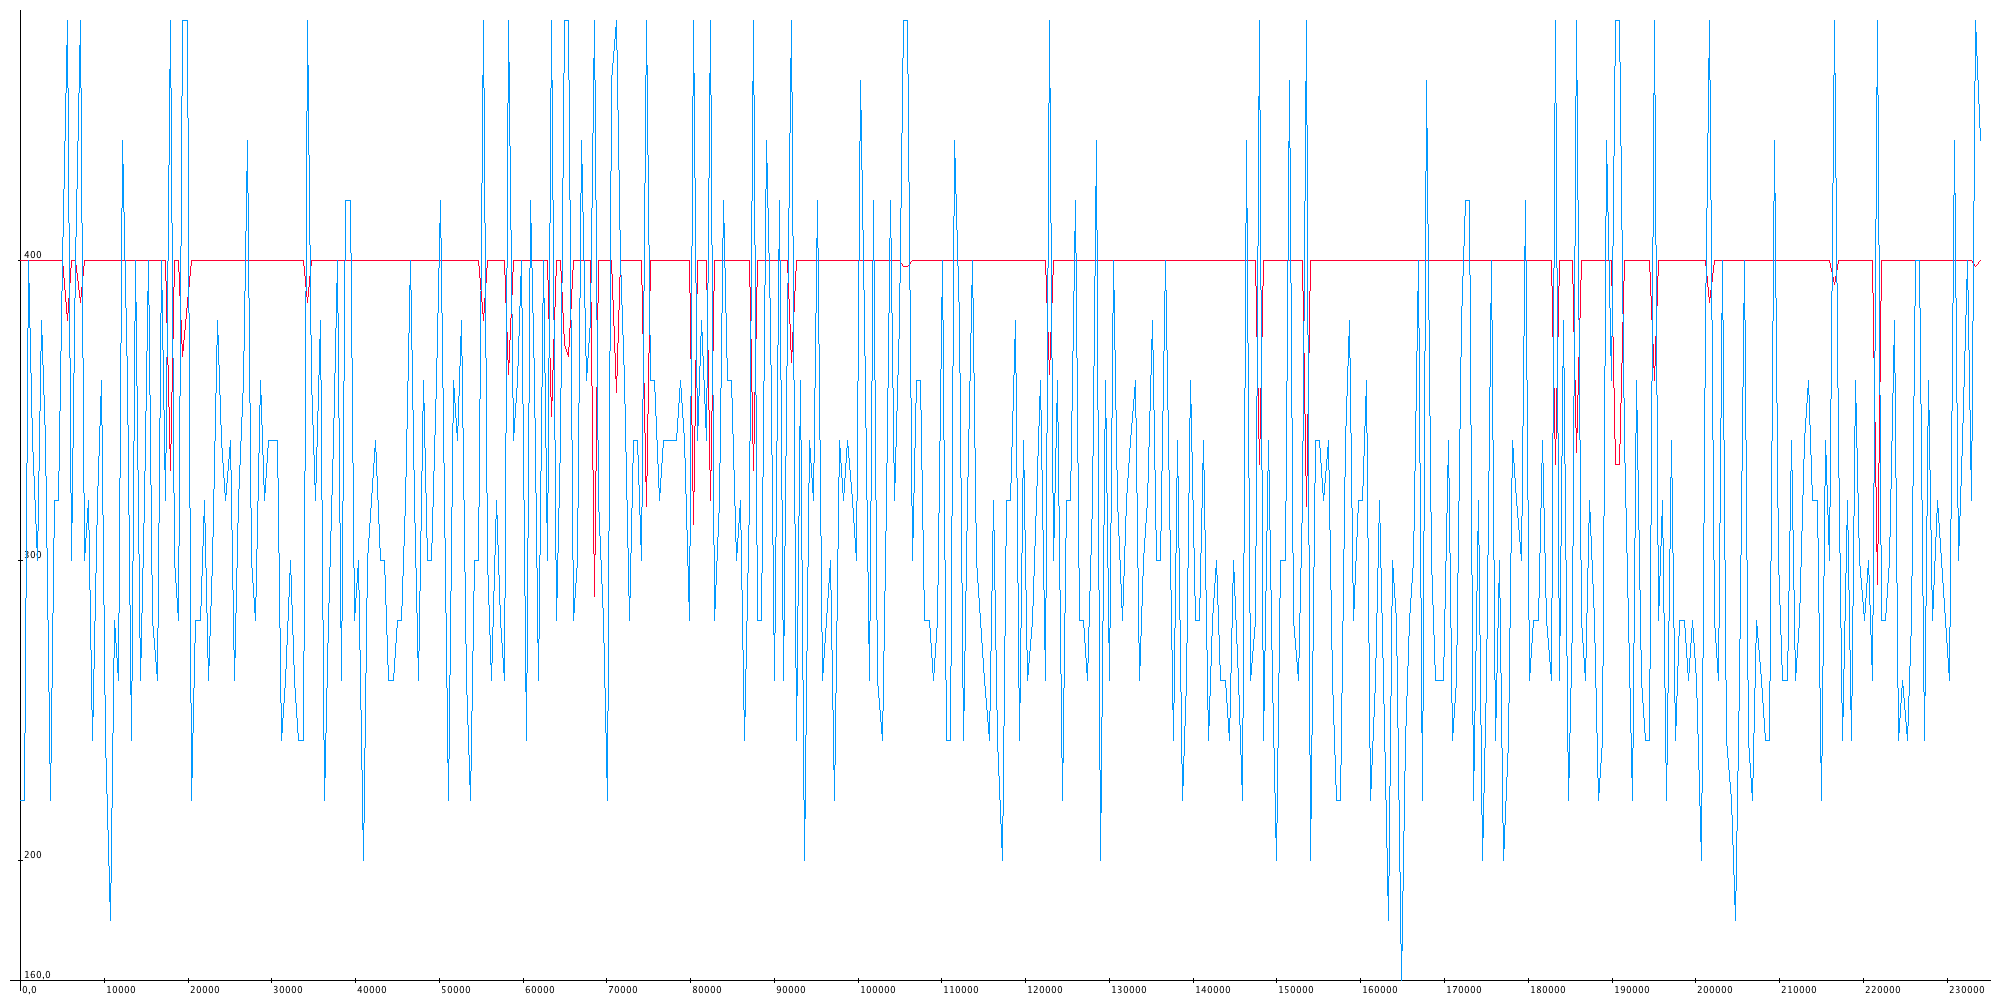
\includegraphics[angle=-90, scale=0.25]{Figures/learningrate/A4G6/damage.png}
\caption{Alpha 4 Gamma 6 damage - Blue: Damage given - Red: Damage taken}
\label{fig:app_a4g6_damage}
\end{figure}	

\begin{figure}[H]
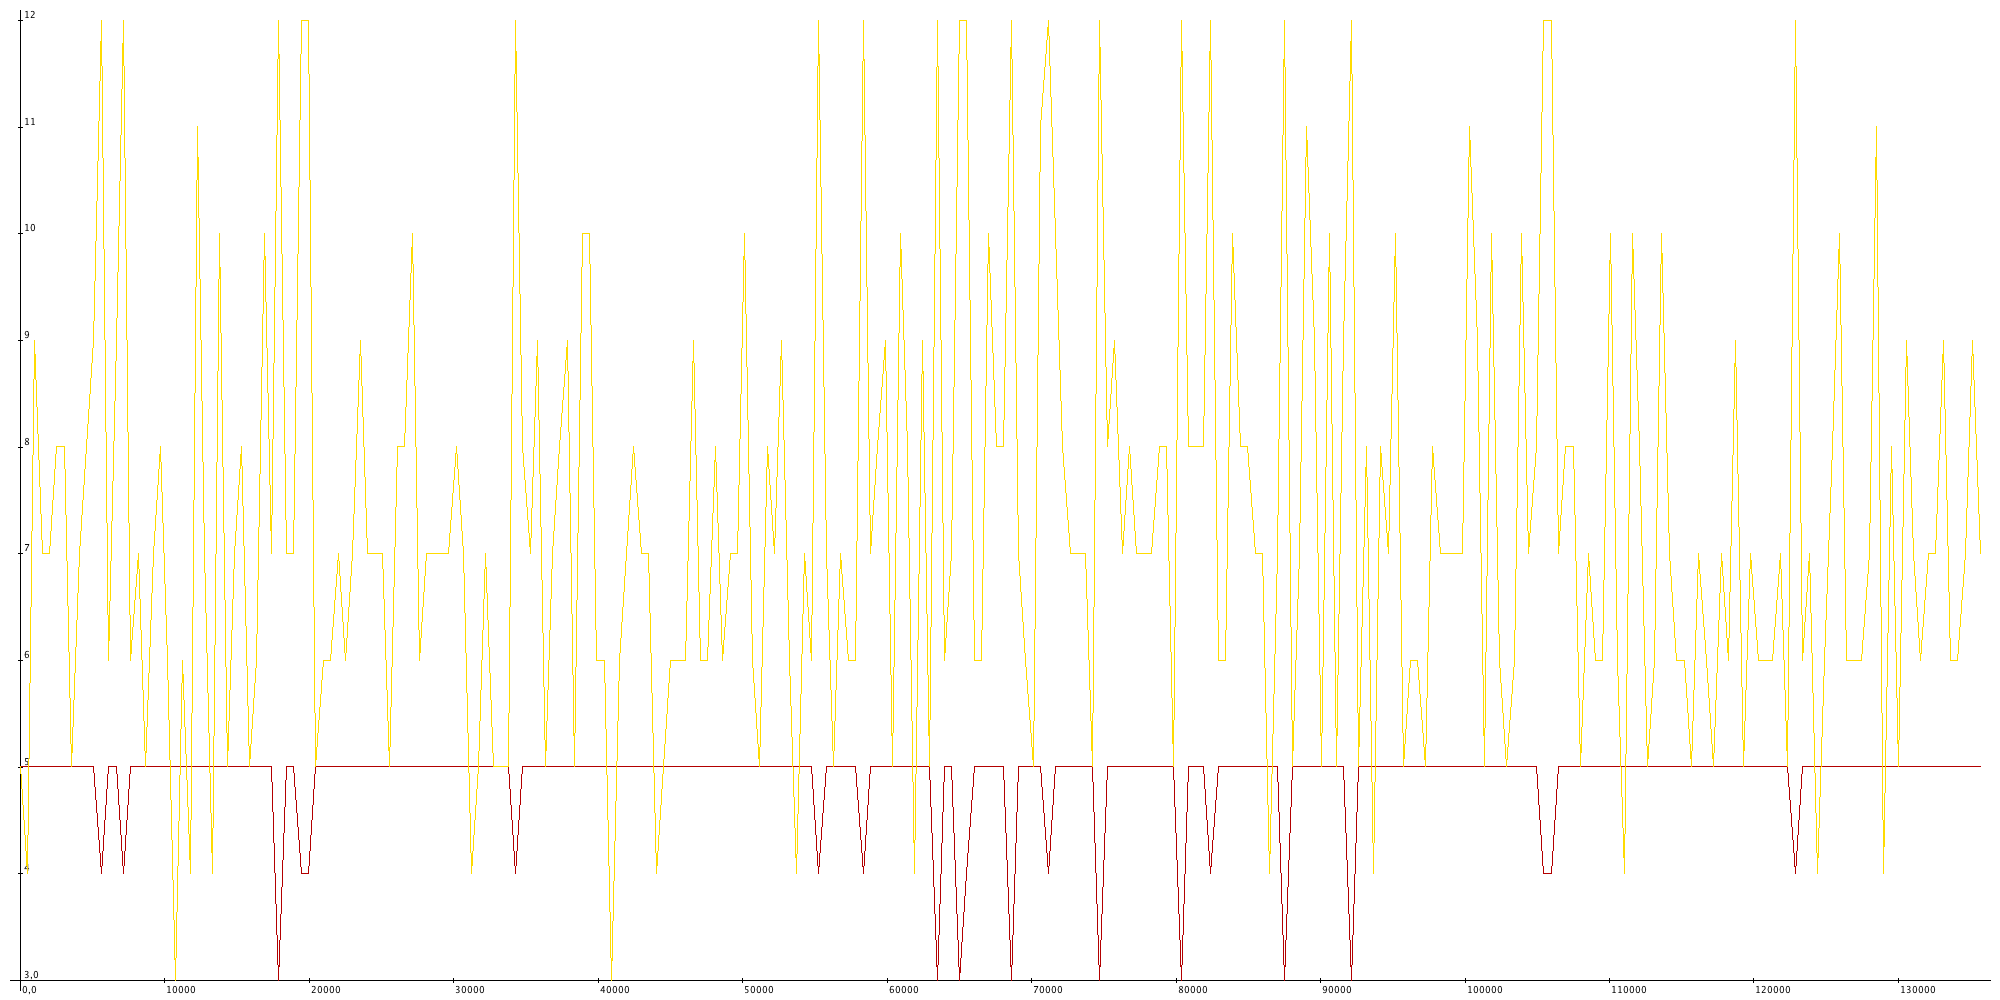
\includegraphics[angle=-90, scale=0.25]{Figures/learningrate/A4G6/units_lost_and_units_killed.png}
\caption{Alpha 4 Gamma 6 units lost and killed - Blue: Enemies killed - Red: Units lost}
\label{fig:app_a4g6_lak}
\end{figure}	

\section{A2G9}
%A2G9
\begin{figure}[H]
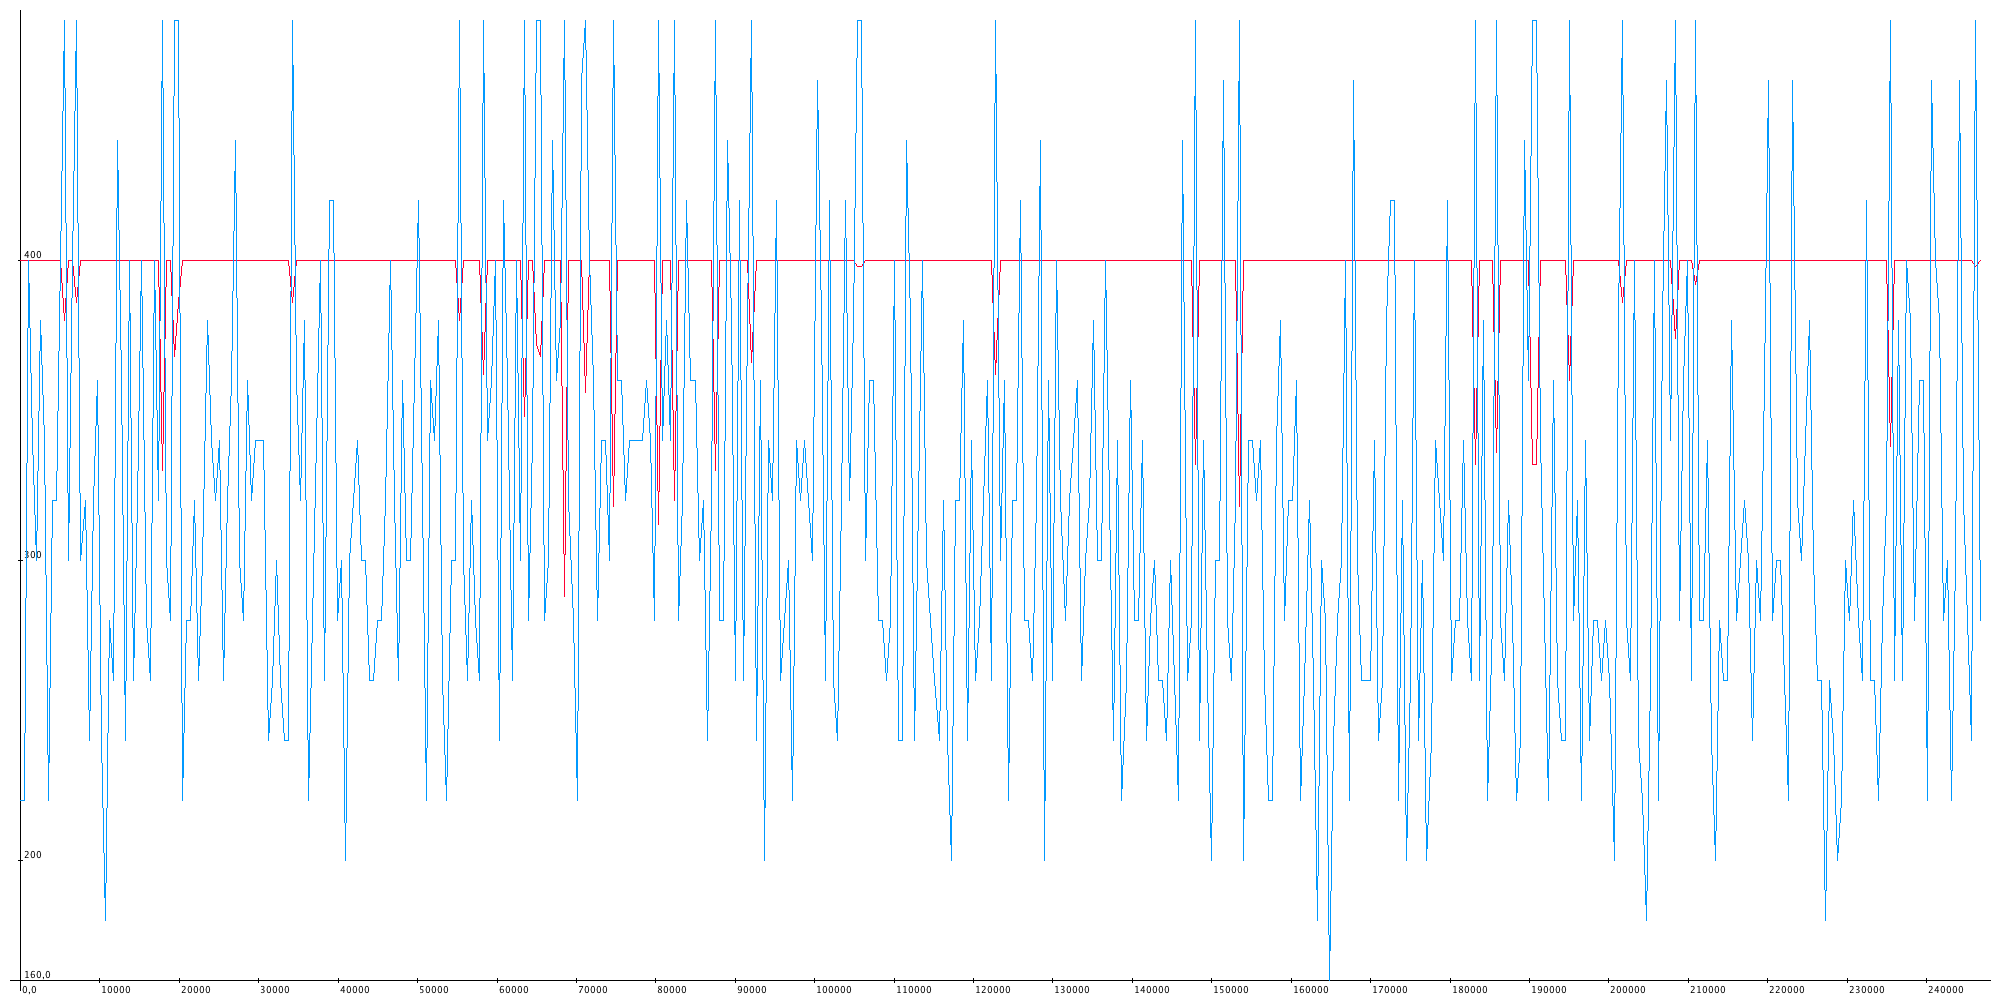
\includegraphics[angle=-90, scale=0.25]{Figures/learningrate/A2G9/damage.png}
\caption{Alpha 2 Gamma 9 damage - Blue: Damage given - Red: Damage taken}
\label{fig:app_a2g9_damage}
\end{figure}	

\begin{figure}[H]
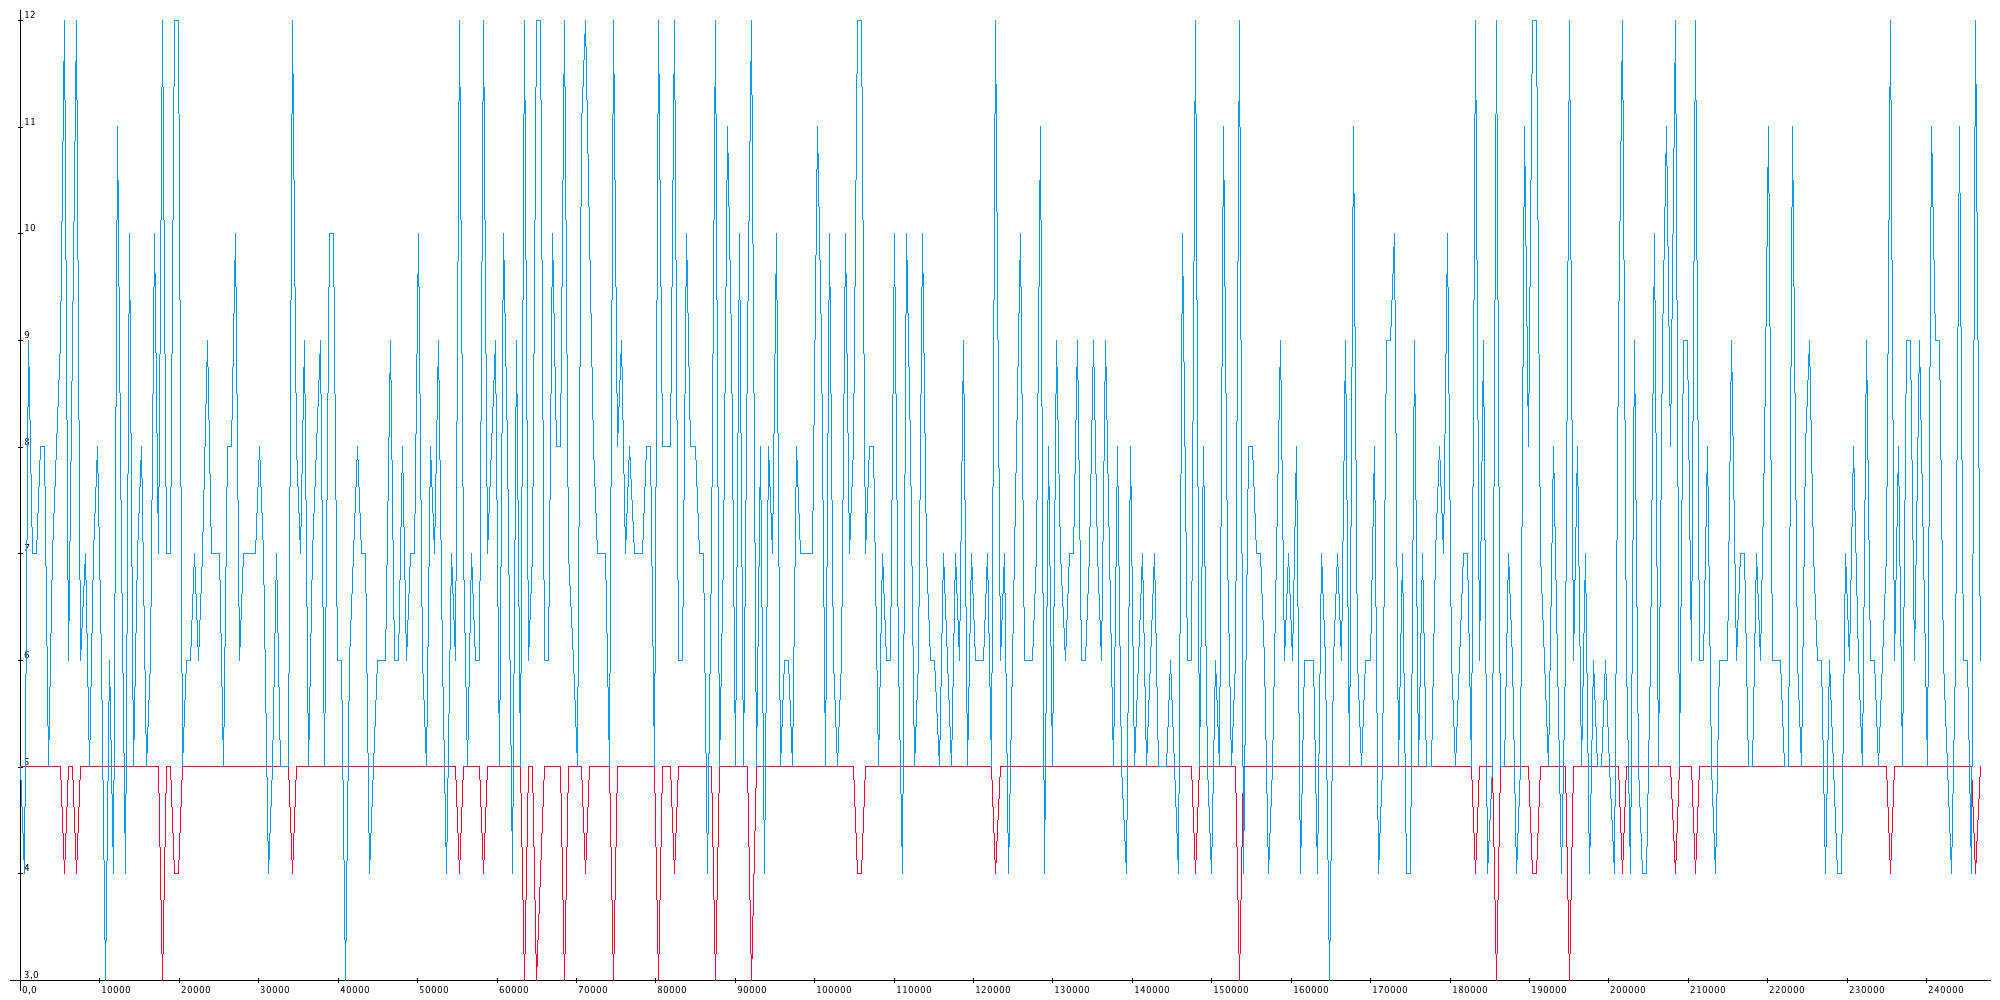
\includegraphics[angle=-90, scale=0.25]{Figures/learningrate/A2G9/units_lost_and_units_killed.png}
\caption{Alpha 2 Gamma 9 units lost and killed - Blue: Enemies killed - Red: Units lost}
\label{fig:app_a2g9_lak}
\end{figure}

%The test.lgdat file from A4G6 (Running on Dans machine)
\begin{figure}[H]
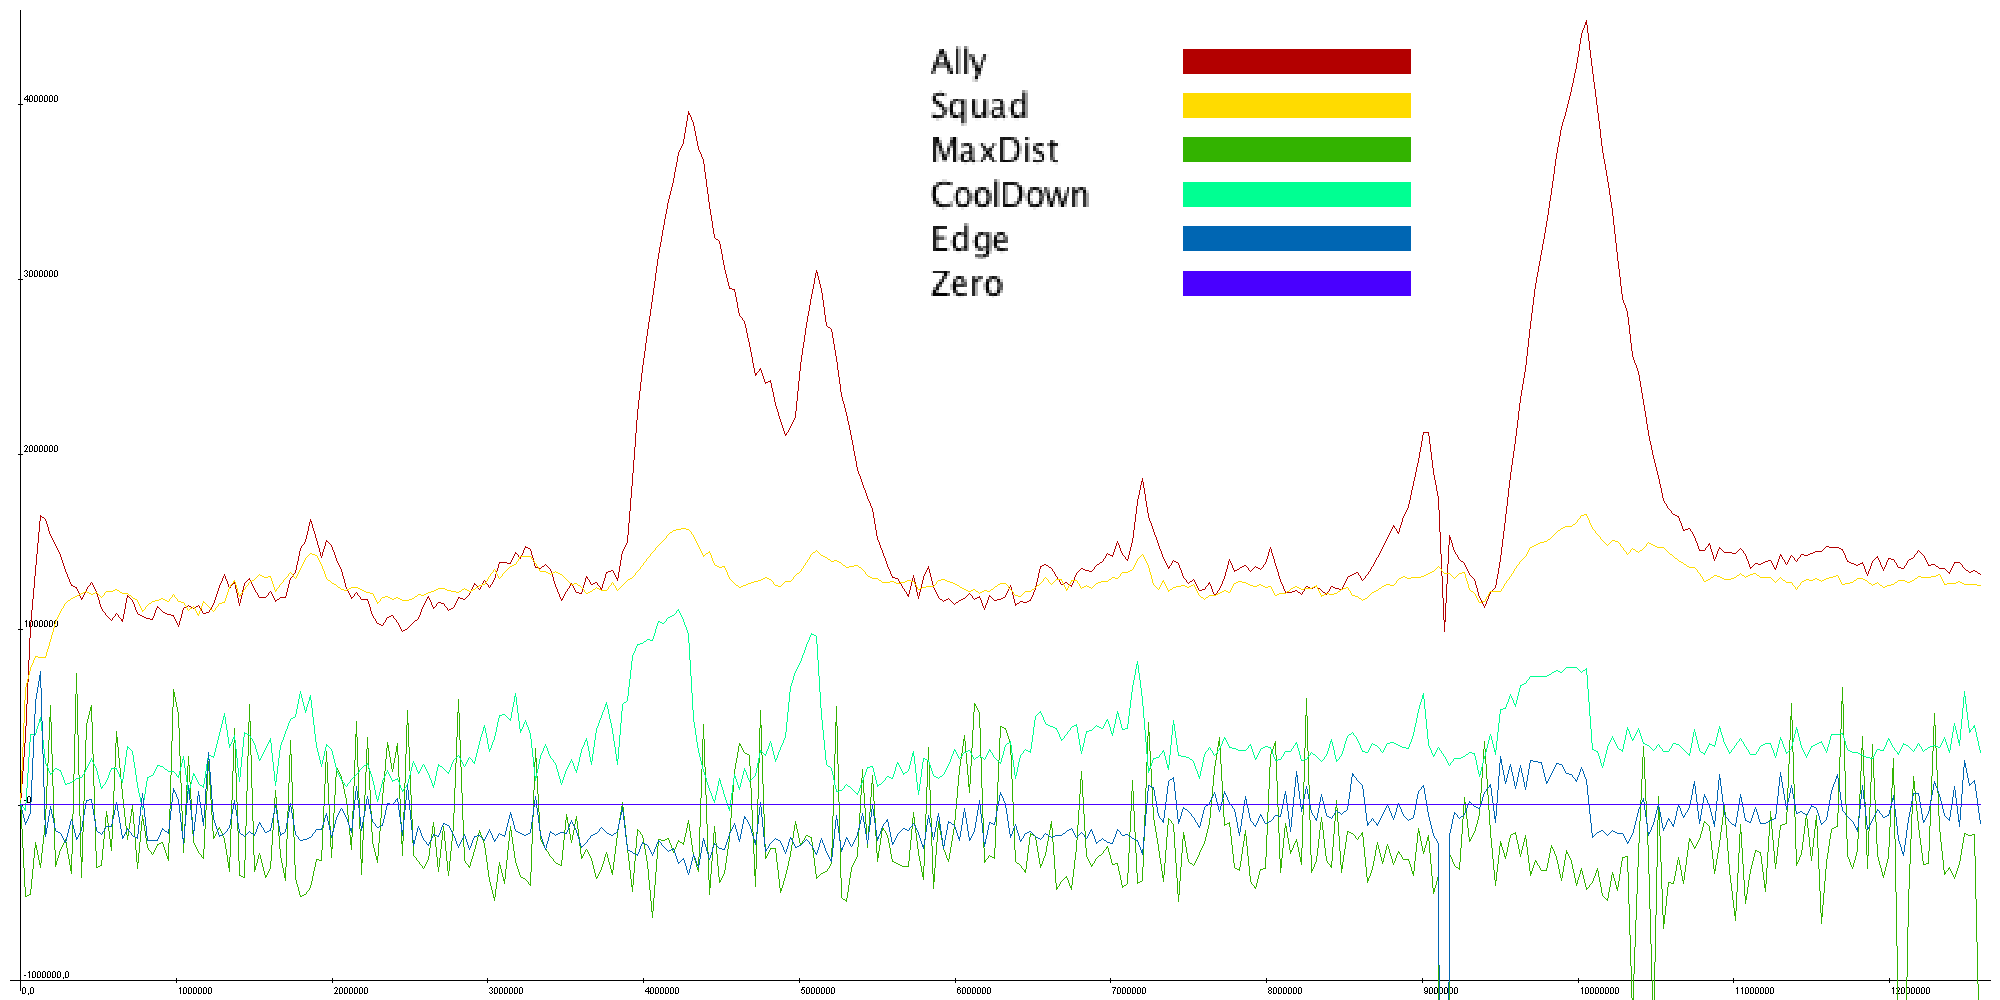
\includegraphics[angle=-90, scale=0.45]{Figures/learningrate/A4G6/test.png}
\caption{Alpha 4 Gamma 6}
\label{fig:app_a4g6_test}
\end{figure}
%The test.lgdat file from A2G9 (Running on grouproom machine)
\begin{figure}[H]
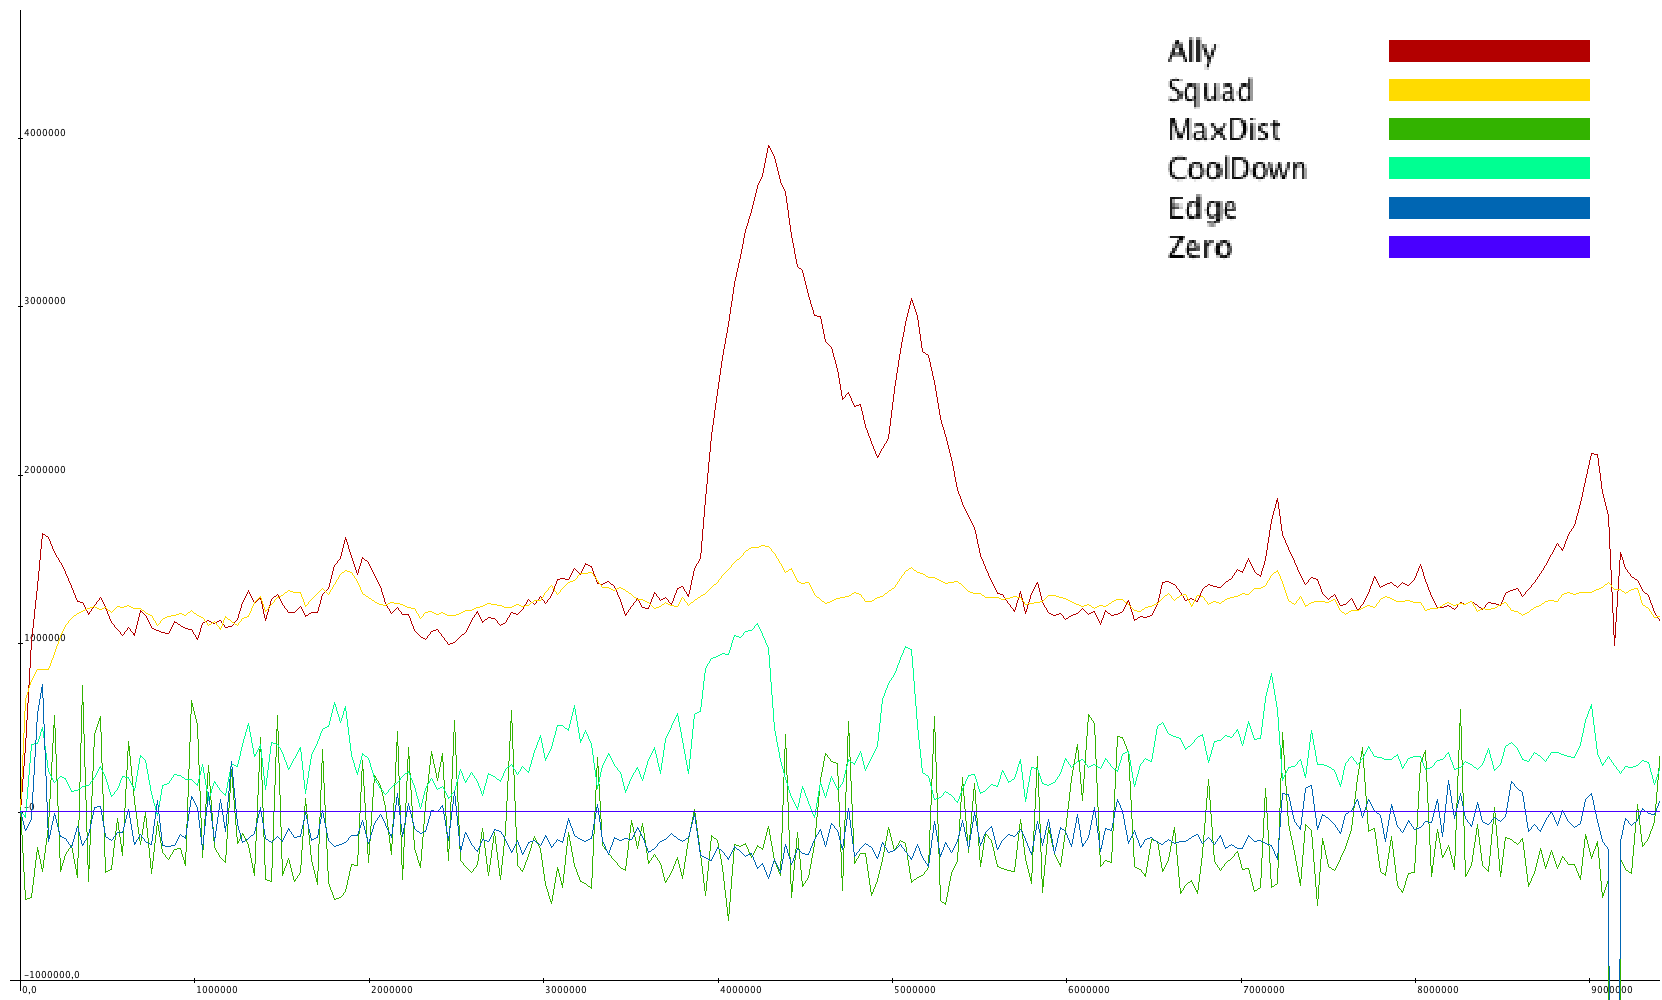
\includegraphics[angle=-90, scale=0.45]{Figures/learningrate/A2G9/test.png}
\caption{Alpha 2 Gamma 9}
\label{fig:app_a2g9_test}
\end{figure}	

\newpage
\section{Winning Streak}
%%Comparing the winning streak%%% done!!
\begin{table}[H]

 \begin{tabular}{|c||c|c|c|c|c|c|}
	\multicolumn{7}{c}{A4G6 winning streak 1} \\
	\hline
	D. taken &			 D. given &		 Ally &		 Squad &		 Max. dist. &		 Cooldown & 		Edge \\
	\hline
	380& 				 		480&						2.39033e+006&1.40153e+006&-282631&			698463&			277493\\
	392& 						480& 					2.39e+006&		1.40181e+006&-278968&			696251&			274540\\
	400& 						300& 					2.39058e+006&1.4019e+006&	-273958&			698558&			279631\\
	400& 						380& 					2.39196e+006&1.40196e+006&-268354&			705666&			293743\\
	368& 						480& 					2.39249e+006&1.40228e+006&-264404&			708283&			296838\\
	400& 						360& 					2.39315e+006&1.40233e+006&-260781&			711552&			301867\\
	400& 						340& 					2.39447e+006&1.40238e+006&-256977&			719614&			312891\\
	324& 						480&						2.39407e+006&1.40262e+006&-256418&			716551&			307314\\
	\hline

\end{tabular}
	\label{winning_streak_A4G6_1_1}
	\caption{First winning streak of A4G6}
\end{table}




\begin{centering}
\begin{table}[H]
 \begin{tabular}{|c||c|c|c|c|c|c|}
	\multicolumn{7}{c}{A4G6 winning streak 2} \\
	\hline
	D. taken & 				D. given & 			Ally & 			Squad & 			Max. dist. & 			Cooldown & 				Edge \\
	\hline
	368& 								480& 					4.09754e+006&	1.551e+006&		-423034&							341397&				-173826\\
	400& 								320& 					4.09229e+006&	1.55017e+006&	-487204&							339150&				-196334\\
	392& 								480& 					4.09461e+006&	1.55022e+006&	-405424&							342703&				-194759\\
	400& 								320& 					4.09038e+006&	1.5499e+006&		-469782&							340807&				-193842\\
	398& 								480& 					4.09328e+006&	1.5499e+006&		-400091&							344188&				-178773\\
	386& 								480& 					4.09453e+006&	1.55029e+006&	-384631&							348976&				-172204\\
	400&		 							340&						4.0933e+006&		1.55037e+006&	-416490&							348259&				-183012\\

	\hline

\end{tabular}
	\caption{Second winning streak of A4G6}
	\label{winning_streak_A4G6_1_2}
\end{table}
\end{centering}



%%Comparing the winning streak%%%
\begin{centering}
\begin{table}[H]

 \begin{tabular}{|c|c|c|c|c|c|c|}
	\multicolumn{7}{c}{A2G9 winning streak 1} \\
	\hline
	D. taken & D. given & Ally & Squad & Max. dist. & Cooldown & Edge \\
	\hline
		398&480& 1.40801e+006&1.574e+006&-761798&281321&298668\\
		362&480&1.40872e+006&1.57429e+006&-756848&287031&305837\\
		400&480&1.4091e+006&1.57471e+006&-752924&288704&310040\\
		400&420&1.40933e+006&1.57481e+006&-749240&288771&312032\\
		400&360&1.40947e+006&1.57496e+006&-745253&289079&313754\\
		400&400&1.40982e+006&1.57511e+006&-742978&290117&314484\\
		400&440&1.40994e+006&1.57522e+006&-739405&290281&316040\\
		368&480&1.41033e+006&1.57547e+006&-733273&293577&323478\\
		282&480&1.4105e+006&1.57584e+006&-802858&293081&311030\\
	\hline
\end{tabular}

	\label{winning_streak_A2G9_1_1}
	\caption{First winning streak of A2G9}
\end{table}
\end{centering}

\newpage


\begin{centering}
\begin{table}[H]
 \begin{tabular}{|c|c|c|c|c|c|c|}
	\multicolumn{7}{c}{A2G9 winning streak 2} \\
	\hline
	D. taken & D. given & Ally & Squad & Max. dist. & Cooldown & Edge \\
	\hline
			374&480&894888&4.65666e+006&-1.94865e+006&12333.4&-96592.9\\
			238&480&895250&4.65597e+006&-1.93662e+006&14373.5&-92902.4\\
			400&300&893479&4.65594e+006&-1.99003e+006&12629.4&-114838\\
			398&480&892553&4.65602e+006&-2.00792e+006&12309.4&-119357\\
			400&280&892857&4.6556e+006&-1.99505e+006&12454.5&-116666\\
			400&480&892257&4.6547e+006&-2.0309e+006&11716.2&-124105\\
	\hline
\end{tabular}
	\label{winning_streak_A2G9_1_2}
	\caption{Second winning streak of A2G9}
	\end{table}
\end{centering}